\chapter{Mapas de comportamiento}\label{cha:mapas_comportamiento}

\AddToShipoutPictureBG*{\put(0,0){%
        \parbox[b][\paperheight]{\paperwidth}{%
            \vfill
            \centering
            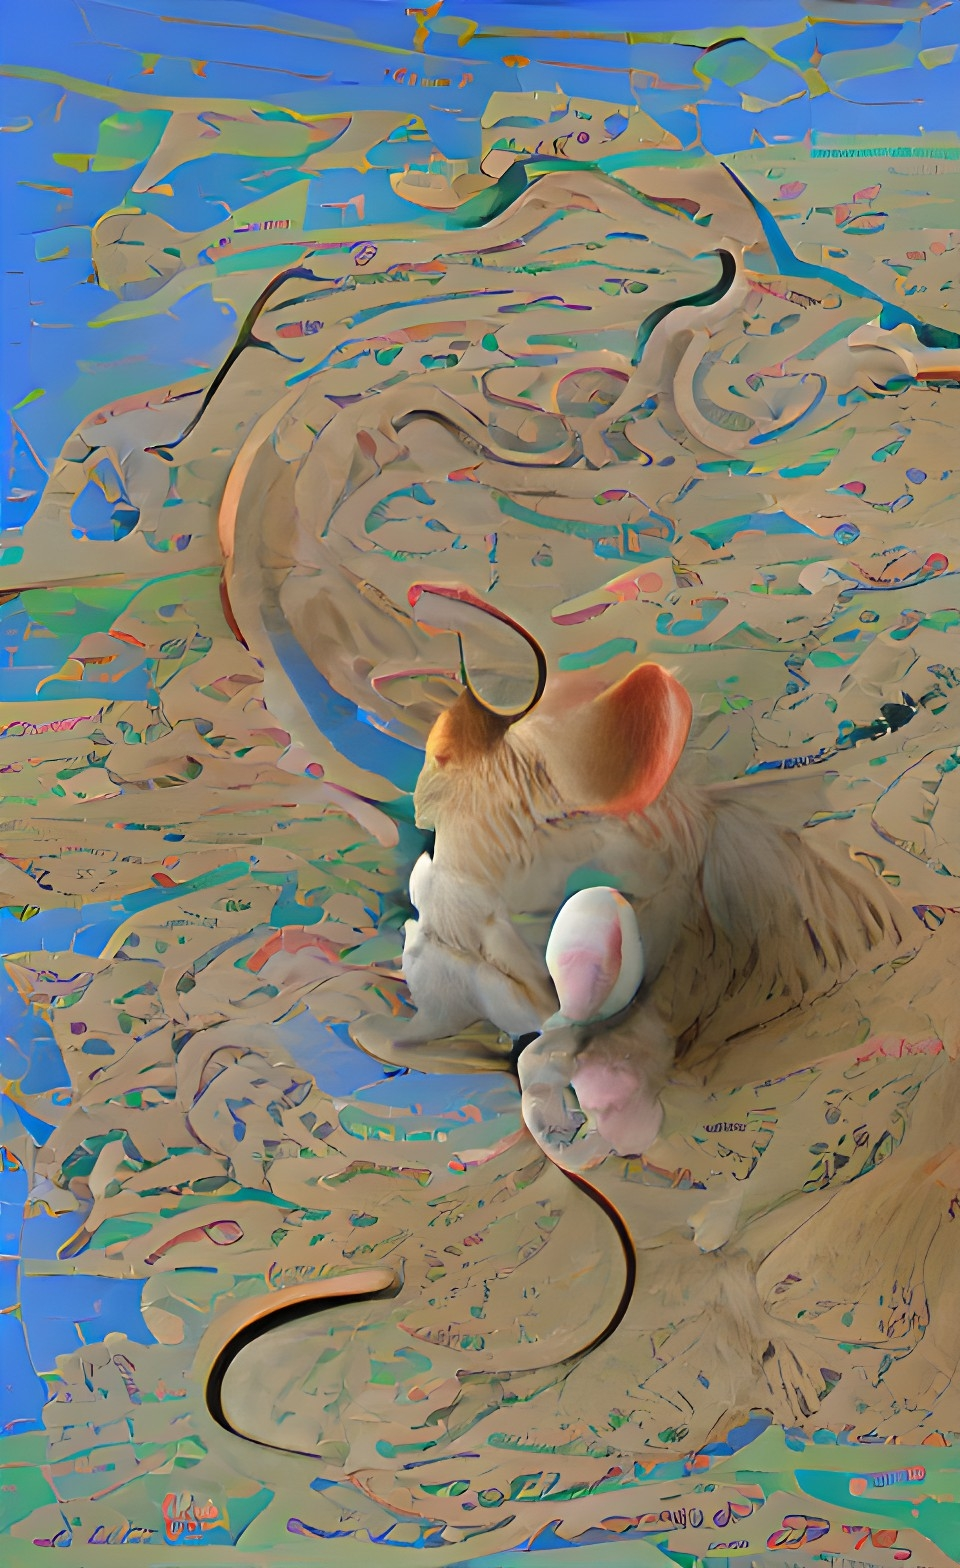
\includegraphics[width=\paperwidth,height=\paperheight,keepaspectratio]{%
                figuras/caratulas/mapa_de_comportamientos.jpg}\vfill
        }}}

\AddToShipoutPicture*{
    \begin{tikzpicture}[overlay, remember picture]
        \fill[white, opacity=0.75] (20, 24) rectangle (1, 21);
    \end{tikzpicture}}

\clearpage

Cuantificar el comportamiento animal es fundamental para el análisis de su correlación con la actividad neuronal con el fin de estudiar cómo el cerebro codifica diferentes comportamientos, cuáles son los circuitos neuronales subyacentes y cómo estos se modifican durante el aprendizaje de nuevas tareas motoras \cite{esposito_defensive, levy_representation}. En general, se necesita una amplia variedad de características para capturar detalladamente las sutilezas del comportamiento animal complejo en un experimento. Debido a que esta alta dimensionalidad en los datos puede resultar inconveniente para su análisis, frecuentemente se utilizan técnicas de reducción de la dimensión sobre los conjuntos de características comportamentales. Estas técnicas generan representaciones de menor dimensión que capturan la mayor parte de la varianza y/o la mayoría de las relaciones de similaridad locales de los datos, es decir, son una buena aproximación del conjunto de datos original. Además, muchas de estas técnicas, como el análisis de componentes principales (\textit{Principal Component Analysis}, PCA), son utilizadas comúnmente en el estudio de registros de actividad neuronal. El algoritmo de PCA identifica un conjunto ordenado de componentes principales (PCs), que constituyen diferentes ejes ortogonales sobre los que se puede descomponer al conjunto de datos. Cada PC captura progresivamente menos varianza en los datos y, por lo tanto, aporta progresivamente menos información, siendo la primera componente principal (PC1) la que captura la mayor proporción de la varianza en los datos. De esta manera, un subconjunto de PCs puede utilizarse para reconstruir de manera aproximada a las características comportamentales subyacentes y usando un menor número de variables en total \cite{datta_computational_neuroethology}.

Sin embargo, por ser una transformación lineal, PCA solo es capaz de capturar relaciones globales a grandes rasgos en la estructura interna de los datos comportamentales. Para respetar mejor la estructura latente del comportamiento a nivel local se pueden utilizar técnicas no lineales de reducción de la dimensión. Algunos de estos algoritmos se basan en construir representaciones que respeten la topología del conjunto de datos original, y luego proyectar esta representación topológica en un espacio de dimensión menor (por lo general en 2 dimensiones, para facilitar su visualización). Estos métodos basados en grafos suelen ser preferibles por encima de los métodos lineales porque capturan la estructura local de los datos, lo cual permite describir detalladamente comportamientos sutiles usando muy pocas dimensiones. Recientemente, la utilidad de estos métodos ha cobrado protagonismo en diversas áreas de investigación en biología y forman parte de las herramientas fundacionales de la neuroetología computacional \cite{sainburg_birdsong_umap}.

En este trabajo, utilizamos proyecciones UMAP (\textit{Uniform Manifold Approximation and Projection}) para describir la actividad de ratones durante la ejecución de la tarea rotarod e inferir categorías comportamentales subyacentes, de manera no supervisada \cite{mcinnes_umap}. El algoritmo UMAP se usó para encontrar proyecciones en 2 dimensiones de conjuntos de datos. La estructura de los datos en este espacio de dimensión baja respeta su estructura topológica latente: dos puntos cercanos en la proyección UMAP son puntos con características similares en el espacio original. Esto se debe a que la proyección UMAP conserva las relaciones de similaridad entre vecinos cercanos en el conjunto de datos (Figuras \ref{fig:capitulo4_labels_umap_wav}a y \ref{fig:capitulo4_labels_umap_stp}a). Consideramos que las regiones del mapa UMAP donde se aglutinan puntos constituyen comportamientos estereotípicos exhibidos por los animales. En etología, el supuesto de estereotipia consiste en que los comportamientos animales pueden ser descompuestos en elementos discretos y reproducibles, y, por lo tanto, pueden representarse en un espacio de dimensión baja. A partir de este supuesto, utilizamos las proyecciones UMAP para explorar estos espacios de comportamientos estereotipados, exhibidos por ratones durante la ejecución y aprendizaje de la tarea rotarod.

Las proyecciones UMAP tienen propiedades similares a las proyecciones LargeVis y t-SNE (\textit{t-Distributed Stochastic Neighbor Embedding}), las cuales son otras herramientas de reducción de la dimensión por medio de grafos y \textit{manifold learning}, que influenciaron fuertemente el desarrollo de UMAP \cite{large_vis, vdm_tsne, kobak_art, kobak_umap_tsne}. La ventaja principal de UMAP es su eficiencia en tiempo de cómputo, al comparar la implementación en Python de \texttt{umap-learn}, con las implementaciones de referencia de t-SNE de \texttt{scikit-learn} y \texttt{openTSNE} \cite{scikit-learn, policar_tsne}. Otra ventaja de la implementación de UMAP es que permite reducir la dimensión de los datos a una dimensión arbitraria, mientras que las implementaciones de t-SNE tienen dificultades para reducir datos a dimensiones mayores a 3, debido a que se vuelve computacionalmente prohibitivo de calcular, incluso usando métodos aproximados.

\begin{figure}[htbp]
    \centering
    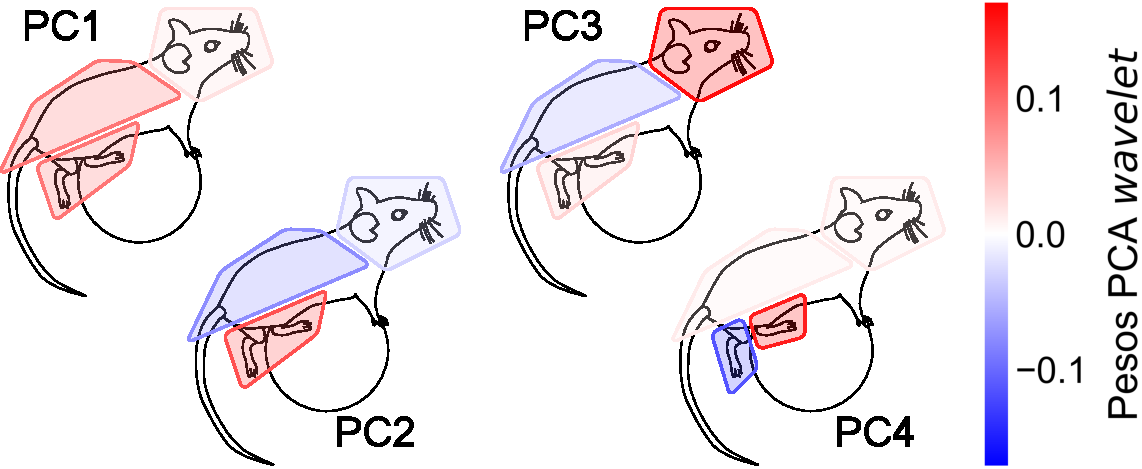
\includegraphics[width=0.8\linewidth]{figuras/capitulo4/partes_del_cuerpo_pca.pdf}
    \caption{\textbf{Pictograma de diferentes modos de locomoción.}
        Ilustración de cómo contribuyen diferentes partes del cuerpo a las 4 primeras componentes principales (PCs) de los espectros \textit{wavelet}. La PC1 consiste en movimientos de todas las partes del cuerpo en proporciones iguales, excepto por la menor participación de la cabeza. La PC2 tiene contribuciones opuestas en los movimientos de las patas respecto de la espalda-cola-nariz. La PC3 está dominada principalmente por movimientos de la cabeza. La PC4 es una locomoción con asimetría entre las patas traseras izquierda y derecha. Para más información sobre los pesos PCA ver \autoref{fig:capitulo4_pesos_pca}}
    \label{fig:capitulo4_partes_del_cuerpo_pca}
\end{figure}

Específicamente, se construyeron 2 mapas UMAP utilizando 2 conjuntos de características comportamentales diferentes. Esto se hizo con la intención de comparar las propiedades de representaciones comportamentales obtenidas a partir de la medición de diferentes aspectos del comportamiento animal. En particular, uno de los mapas se construyó a partir de las primeras 50 componentes principales (Figuras \ref{fig:capitulo4_partes_del_cuerpo_pca} y \ref{sec:apendice_pca_wavelet}) de los espectros \textit{wavelet} de los movimientos de los ángulos entre partes del cuerpo de los ratones, las cuales capturan el 84\% de la varianza de los datos. Esto se hizo para facilitar el cómputo de la proyección UMAP: el cálculo de UMAP a partir de 50 componentes principales puede realizarse en una computadora personal, mientras que el cálculo de UMAP a partir de las 500 variables que describen los espectros \textit{wavelet} requiere mayor memoria.

Por su parte, el segundo mapa UMAP se construyó a partir de las características que describen los pasos y las poses de los ratones (\autoref{fig:capitulo4_caracteristicas_pasos_poses}). Adicionalmente, las características de los pasos se promediaron entre las patas izquierda y derecha de los ratones, para eliminar diferencias por pata dominante de los ratones, mientras que las características de las poses, es decir, las posiciones de los marcadores de las partes del cuerpo, se procesaron para eliminar también diferencias por lateralidad en los ratones. Más en detalle: se relativizaron las posiciones de los marcadores respecto al centro de masa de los ratones y se calculó el valor absoluto de sus coordenadas horizontales; similarmente, la coordenada horizontal del centro de masa de los ratones se relativizó al centro del compartimento del rotarod donde se ubica el ratón, y se calculó su valor absoluto; y, finalmente, las coordenadas de las patas izquierda y derecha se reemplazaron por nuevas variables calculadas a partir de la diferencia y el promedio en las posiciones de las patas. De esta manera, se quitó efectivamente toda distinción entre izquierda y derecha en las características, volviendo indistinguibles ratones diestros de zurdos. Esto se hizo porque en el análisis no supervisado de comportamiento que se realizó anteriormente, en el trabajo de licenciatura, se observaron diferencias entre individuos asociadas a su lateralidad.

Debido a la complejidad en memoria del algoritmo UMAP, el cómputo de los mapas debe hacerse sobre una muestra parcial del conjunto de datos. Para cada conjunto de características se tomaron muestras aleatorias de datos con la misma densidad de probabilidad que la densidad de pasos ejecutados por el ratón en el tiempo. Es decir, los intervalos de tiempo en los que el ratón dio una mayor cantidad de pasos fueron muestreados con mayor frecuencia que otros intervalos de tiempo, de igual duración, pero con un menor número de pasos registrados. Esto se hizo para representar mejor la actividad del ratón, siguiendo la escala de tiempo natural de su comportamiento: los tiempos de sus pasos.

En resumen, el mapa UMAP de las componentes principales de los espectros \textit{wavelet} (\autoref{fig:capitulo4_umap_wav}) se construyó con 255\,060 puntos (4.7\% del total) y el mapa UMAP de las características de pasos y poses (\autoref{fig:capitulo4_umap_stp}) se construyó con 509\,995 puntos (9.3\% del total). Ambos mapas se construyeron usando similaridad coseno como noción de distancia en el espacio original de los datos, y con parámetros del \textit{kernel} de densidad en el espacio de dimensión baja $a=1.0$ y $b=0.4$. El mapa UMAP \textit{wavelet} se construyó con $n_{\mathrm{neighbors}}=100$ y el mapa de pasos y poses con $n_{\mathrm{neighbors}}=30$. Se utilizó un mayor número de vecinos cercanos en el mapa \textit{wavelet} para compensar por el mayor tiempo de autocorrelación de estas características, y permitir que se formen relaciones de similaridad entre los datos por fuera de su autocorrelación temporal (\autoref{fig:capitulo4_componentes_pca}). Esto no fue necesario para el mapa de pasos y poses, donde se usó el número de vecinos por defecto, ya que estas características tienen menores tiempos de autocorrelación (\autoref{fig:capitulo4_caracteristicas_pasos_poses}). Finalmente, para mapear el resto de los puntos que no fueron muestreados al construir las proyecciones UMAP se utilizó un clasificador $k$-NN (\textit{k-Nearest Neighbors}) con $k=5$ vecinos cercanos. De esta manera, se obtuvieron las proyecciones UMAP de 5\,458\,552 puntos en total, representando cada uno de estos un instante de tiempo de un ratón ejecutando una prueba rotarod en particular.

\section{Estructura espacial y temporal de los mapas}\label{sec:umap_trans}

Para obtener categorías que aglutinen comportamientos similares (\textit{labels}) se realizaron segmentaciones \textit{watershed} de los mapas UMAP. Este algoritmo no requiere que se defina \textit{a priori} un número fijo de regiones a encontrar. El espacio UMAP está formado por picos y valles de densidad de puntos. La segmentación \textit{watershed} encuentra áreas conexas del mapa que encierren estos picos de densidad de puntos y estén separadas entre sí por los valles de baja densidad \cite{meyer_watershed_history, compact}. Para obtener esta segmetanción se calcularon las densidades de probabilidad de los puntos en los mapas UMAP usando \texttt{fastKDE}, una herramienta para estimación rápida de densidad de probabilidad implementada en Python \cite{obrien_fastkde}, mientras que la segmentación \textit{watershed} se realizó con el paquete \texttt{scikit-image} \cite{scikit-image}. Se utilizó este algoritmo de segmentación por su eficiencia computacional para procesar conjuntos de datos bidimensionales de millones de puntos. Al terminar este proceso se obtuvieron 10 \textit{labels} de comportamiento para cada mapa. Los parámetros del algoritmo de segmentación se pueden ajustar para realizar particiones más finas o más gruesas del mapa. En nuestro caso decidimos mantener el número de regiones encontradas entre 5 y 20 para facilitar el análisis, por lo que afinamos los parámetros del algoritmo para este fin. De hecho, existen otros algoritmos de segmentación, por ejemplo HDBSCAN (\textit{Hierarchical Density-Based Spatial Clustering of Applications with Noise}), que permiten obtener segmentaciones en categorías jerarquizadas con diferentes niveles de detalle \cite{hdbscan}. Sin embargo, la eficiencia computacional de la simple segmentación \textit{watershed} fue más conveniente. Para poder utilizar una herramienta de segmentación jerárquica como HDBSCAN es necesario trabajar con una muestra de alrededor de 100\,000 datos o menos, debido a su complejidad computacional en memoria.

\begin{figure}[htbp]
    \centering
    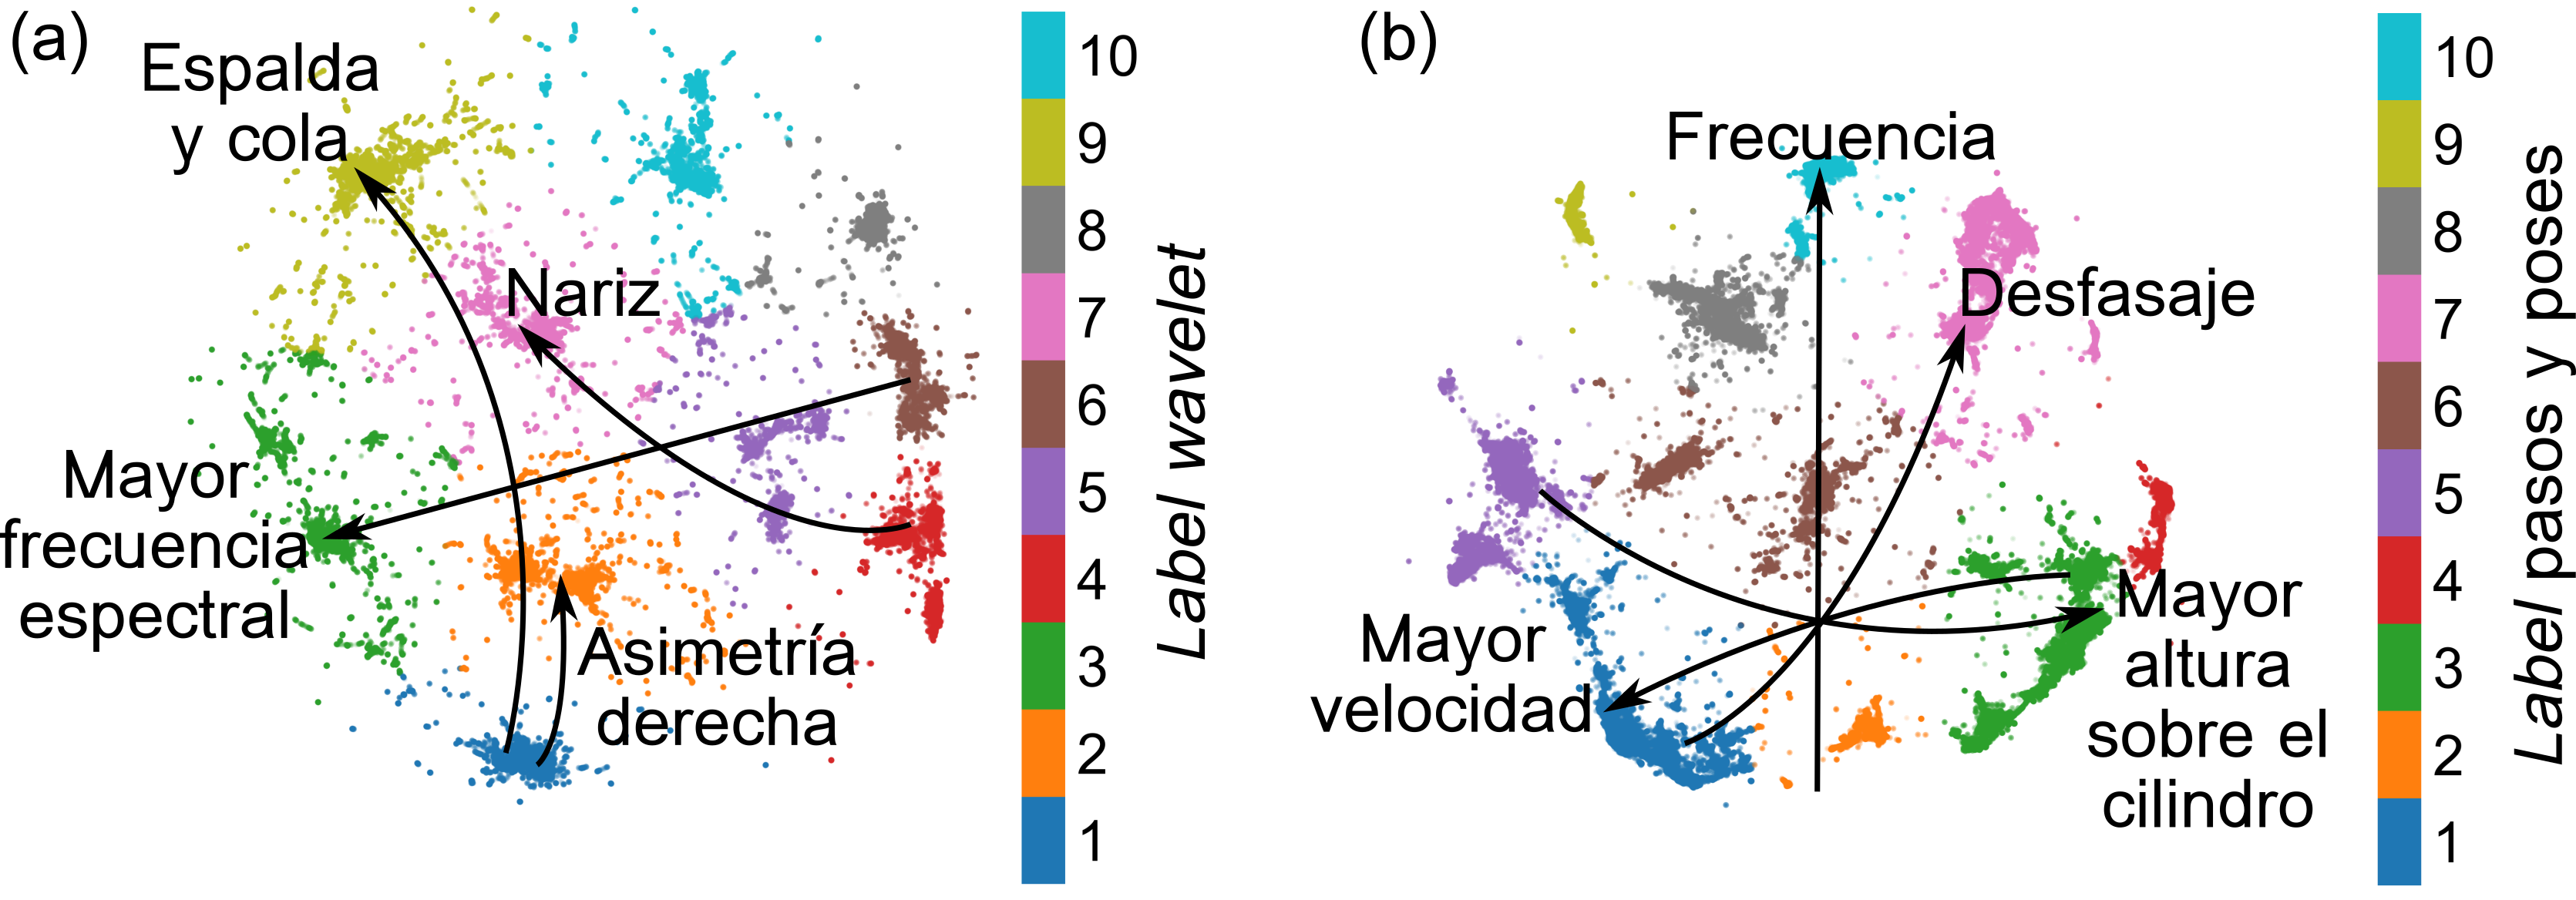
\includegraphics[width=0.99\linewidth]{figuras/capitulo4/comentario_label_umap.png}
    \caption{\textbf{Descripción de las propiedades de los comportamientos de cada mapa.}
        Las flechas indican, de manera simplificada, el sentido en que aumentan diferentes propiedades sobre el mapa. (a) Proyección UMAP de las primeras 50 componentes principales de los espectros \textit{wavelet} de partes del cuerpo del ratón. Se observan regiones en el mapa con diferente frecuencia promedio espectral, y diferencias en los movimientos de la espalda-cola, nariz y asimetría entre patas traseras derecha e izquierda. (b) Proyección UMAP de las características de pasos y poses. Se observan regiones del mapa con diferentes frecuencias de pasos, desfasajes, velocidades y alturas a las que el ratón se posiciona sobre el cilindro.}
    \label{fig:capitulo4_comentario_label_umap}
\end{figure}

Ocasionalmente, estos métodos no supervisados de clasificación pueden resultar en categorías de comportamiento difíciles de reconocer por parte de un humano o de describir en pocas palabras \cite{datta_computational_neuroethology, berman_mapping}. Esto suele ocurrir más frecuentemente en las representaciones de comportamientos complejos. De todas formas, podemos intentar describir en términos generales algunos aspectos de cada label (\autoref{fig:capitulo4_comentario_label_umap} obtenida a partir del análisis de las Figuras \ref{fig:capitulo4_umap_wav} y \ref{fig:capitulo4_umap_stp} suplementarias). Por ejemplo en el mapa UMAP \textit{wavelet} (\autoref{fig:capitulo4_comentario_label_umap}a), podemos observar que los \textit{labels} 4, 5, 6, 8 y 10 tienen menores valores de la primera componente principal (PC1, en la \autoref{fig:capitulo4_umap_wav}a) de los espectros \textit{wavelet} que los \textit{labels} 1, 2, 3, 7 y 9. La PC1, a su vez, acompaña a la frecuencia espectral promedio del movimiento de todas las partes del cuerpo (\autoref{fig:capitulo4_partes_del_cuerpo_pca}), por lo que está asociada a qué tan rápido se mueven las partes del cuerpo de los ratones. Haciendo un análisis similar, y observando los valores de la segunda componente principal (\autoref{fig:capitulo4_umap_wav}b), deducimos que el \textit{label} 9 está asociado a un tipo de locomoción con mucho movimiento en la espalda y en la cola, relativo al movimiento de las patas traseras, mientras que para el \textit{label} 1 se observa la situación opuesta. Usando la tercera componente principal (\autoref{fig:capitulo4_umap_wav}c), asociamos al \textit{label} 7 con locomoción con mucho movimiento de la nariz y la cabeza del animal. Finalmente, el \textit{label} 2 está asociado a un mayor movimiento de la pata trasera derecha que la izquierda, y se observa lo opuesto para el \textit{label} 1, mientras que para el resto de \textit{labels} la asimetría es menos perceptible (\autoref{fig:capitulo4_umap_wav}d).
Por su parte, en el mapa UMAP de pasos y poses (\autoref{fig:capitulo4_comentario_label_umap}b), observamos que los \textit{labels} 3, 4, 7 y 10 corresponden a estrategias donde los pasos de las patas traseras se realizan a una altura elevada sobre el cilindro rotarod, mientras que los \textit{labels} 1, 5 están asociados a pasos en la parte más baja del cilindro (\autoref{fig:capitulo4_umap_stp}a). Respecto a las velocidades promedio de los pasos (\autoref{fig:capitulo4_umap_stp}b), los \textit{labels} 2, 3, 4 y 10, junto con una parte del 6 y del 7, son de baja velocidad de pasos, mientras que los \textit{labels} 1, 5 y 8, junto con la otra parte del 6 y del 7, son de mayor velocidad de pasos. En cuanto al desfasaje entre las patas traseras (\autoref{fig:capitulo4_umap_stp}c), el \textit{label} 7 está asociado a pasos con gran desfasaje y los \textit{labels} 1 y 3 presentan parcialmente puntos con bajo desfasaje. Quizá la relación más clara sea la de la frecuencia con la que el ratón da pasos (\autoref{fig:capitulo4_umap_stp}d), la cual aumenta gradualmente desde abajo hacia arriba en el espacio UMAP, siendo los \textit{labels} 1, 2, 3 y 4 los de menor frecuencia y los \textit{labels} 9 y 10 de mayor frecuencia.

Una de las razones por las que realizamos dos proyecciones UMAP a partir de diferentes conjuntos de características para describir el comportamiento es para estudiar qué tanta información tienen en común ambas representaciones. Ya que no siempre es claro qué características comportamentales son más relevantes o informativas \textit{a priori} y muchas veces se identifican características inesperadas potencialmente útiles de esta manera. Una vez obtenidos los \textit{labels} de comportamiento en el UMAP \textit{wavelet} y en el UMAP pasos y poses, calculamos el valor de la información mutua ajustada entre las dos segmentaciones de datos, usando la implementación en Python de \texttt{scikit-learn} \texttt{metrics.adjusted\_mutual\_info\_score} \cite{scikit-learn, adjusted_mutual_info_score}. Esta es una medida de qué tan similares son ambas maneras de categorizar el comportamiento de los ratones. Este valor puede estar entre 0 y 1, con 0 correspondiendo a segmentaciones completamente independientes entre sí (es decir, cada una aportaría información nueva sobre el comportamiento) y con 1 correspondiendo a segmentaciones equivalentes desde el punto de vista de la información nueva que aportan. En nuestro caso, la información mutua ajustada entre las segmentaciones es de 0.22, el cual es un valor relativamente bajo, pero no insignificante. Esto quiere decir que las dos maneras propuestas para representar el comportamiento animal aportan información novedosa entre sí. Esto tiene sentido, pues los espectros \textit{wavelet} de los ángulos de las partes del cuerpo de los ratones aportan información principalmente sobre la dinámica de sus movimientos, mientras que las características de los pasos y las poses de los ratones aportan mayormente información sobre las posiciones de sus partes del cuerpo en el espacio en un dado instante.

Esto da paso a la pregunta, ¿qué pasaría si combinamos las características dinámicas de los \textit{wavelets} con las características de los pasos y poses en una misma representación del comportamiento? Nuestra hipótesis es que un tipo de características dominará sobre el resto en la representación. Esto se debe, por un lado, a que las proyecciones UMAP tienen que comprometer ciertos aspectos de los datos para poder representarlos en solo dos dimensiones, y, por otro lado, en el momento en que realizamos una segmentación \textit{watershed} de los mapas estamos eligiendo un nivel de detalle en nuestros \textit{labels}. Esto obligaría a que se priorice un tipo de características comportamentales por sobre las demás, mientras que el resto de características podrían influir en la estructura más fina y detallada de los mapas comportamentales. Esta sería una situación interesante para aplicar una segmentación jerárquica, por ejemplo HDBSCAN, para tener acceso a representaciones más finas del comportamiento y conocer su ordenamiento. Sin embargo, esto también haría que el análisis sea mucho más complejo, pasando por diferentes escalas de detalle. De todas formas, en este trabajo se realizó una especie de prueba piloto al combinar varios tipos de características en una proyección UMAP: las características de pasos y poses. Un análisis de información mutua de los \textit{labels} de pasos y poses con sus características correspondientes revela que un tipo de característica (específicamente los valores en los eventos de pasos) aporta mucha más información acerca de estos \textit{labels} que las demás variables (\autoref{fig:capitulo4_mi_labels_scaler_stp}). Esto apoya nuestra hipótesis de que al usar varios tipos de características heterogéneas, alguno de estos tipos termina dominando sobre los demás, por lo menos al usar un nivel de detalle similar al presentado en nuestro análisis.

Otra cuestión interesante es investigar la estructura temporal de los \textit{labels} obtenidos. Por ejemplo, ver qué \textit{labels} se utilizan más comúnmente al iniciar y al terminar una prueba rotarod. Dado que los \textit{labels} tienen duraciones variables (Figuras \ref{fig:capitulo4_labels_umap_wav}c y \ref{fig:capitulo4_labels_umap_stp}c), el estudio de su probabilidad de ocurrencia, sin corregir por su duración, podría traer como consecuencia una sobre-representación de los \textit{labels} que duren más en cada una de sus apariciones. Para reducir estas diferencias debido a la variabilidad de las duraciones, definimos secuencias condensadas de \textit{labels} agrupándolos en bloques consecutivos de una misma categoría comportamental y considerando cada uno de estos bloques como una única observación del \textit{label}. De esta manera resultan secuencias de \textit{labels} sin repeticiones consecutivas de una misma categoría de comportamiento, para las que reservaremos la denominación de ``secuencias'', para diferenciarlas de las ``series temporales'' de \textit{labels} de donde provienen. Con estas secuencias de \textit{labels}, sin repeticiones consecutivas, construimos los grafos de transiciones temporales de cada mapa UMAP (Figuras \ref{fig:capitulo4_labels_umap_wav}b y \ref{fig:capitulo4_labels_umap_stp}b). Adicionalmente, utilizando los 5 primeros y 5 últimos \textit{labels} observados en las secuencias comportamentales de cada prueba calculamos las probabilidades de transiciones desde el estado ``inicio'' y hacia el estado ``fin'' de la prueba. Para cada mapa UMAP se observan conjuntos distintos de \textit{labels} que se observan con mayor frecuencia en el inicio o en el final de cada prueba rotarod. Al iniciar cada prueba, es más probable que un ratón ejecute los comportamientos 6, 8, 9 y 10 del mapa \textit{wavelets} (\autoref{fig:capitulo4_labels_umap_wav}b), o los comportamientos 1, 2, 3, 4 y 6 del mapa pasos y poses (\autoref{fig:capitulo4_labels_umap_stp}b). Mientras que antes de terminar una prueba, es más probable observar los comportamientos 1, 2 y 3 del mapa \textit{wavelets} (\autoref{fig:capitulo4_labels_umap_wav}b), o los comportamientos 1, 5, 6, 8 y 9 del mapa pasos y poses (\autoref{fig:capitulo4_labels_umap_stp}b).

Finalmente, nos preguntamos si la estructura espacial de las proyecciones UMAP tiene alguna relación con la estructura temporal de las secuencias de comportamientos. Esto puede observarse en primera instancia en los grafos de transiciones (Figuras \ref{fig:capitulo4_labels_umap_wav}b y \ref{fig:capitulo4_labels_umap_stp}b). Resulta que las transiciones temporales más probables se producen entre regiones colindantes en el mapa, tanto para el mapa \textit{wavelet} como para el mapa de pasos y poses. Más aún, se observa la existencia de una estructura espacial más fina si coloreamos los mapas UMAP según el \textit{label} que le sigue a cada punto en la secuencia de comportamiento (Figuras \ref{fig:capitulo4_labels_umap_wav}d y \ref{fig:capitulo4_labels_umap_stp}d). Efectivamente, dentro de cada región segmentada de los mapas se observan estructuras más finas donde hay una mayor preferencia por transiciones temporales hacia un tipo particular de \textit{label} por sobre los demás.

\begin{figure}[htbp]
    \centering
    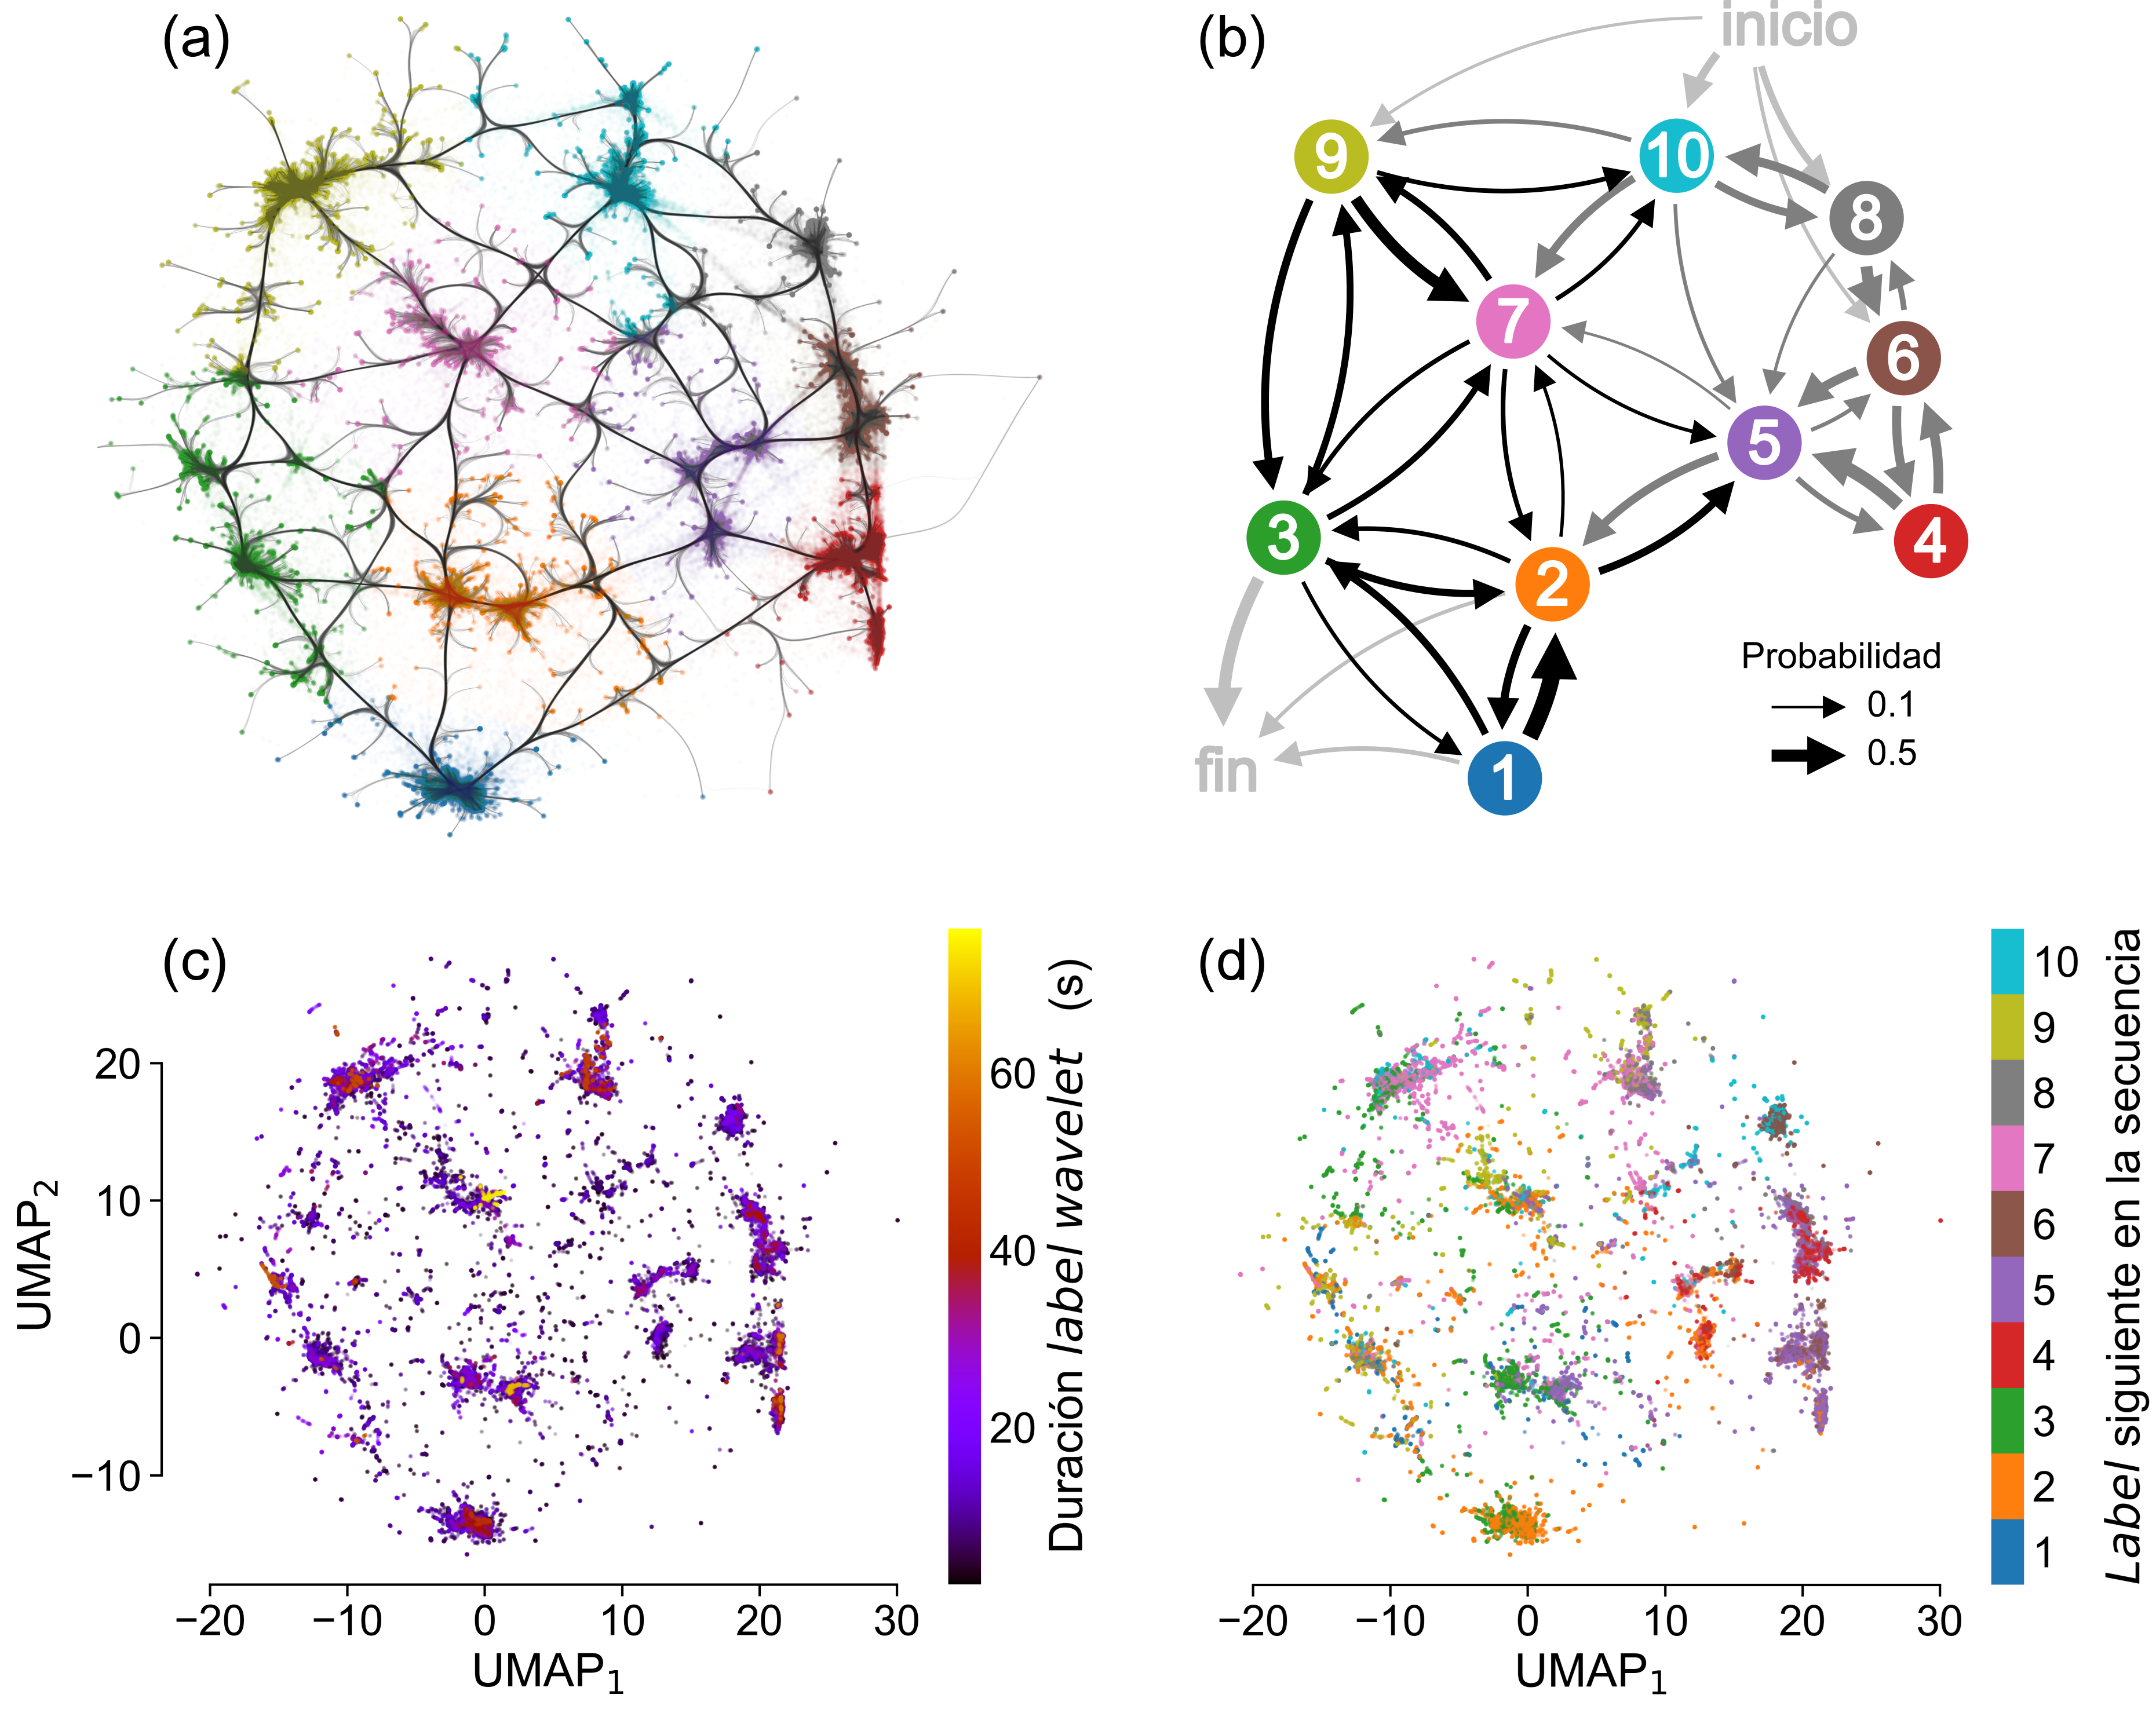
\includegraphics[width=0.99\linewidth]{figuras/capitulo4/labels_umap_wav.png}
    \caption{\textbf{\textit{Labels} de comportamiento de la proyección UMAP de las componentes principales de los espectros \textit{wavelet}.}
        (a) Similaridad entre los puntos del mapa. El grosor de cada línea es proporcional a la similaridad entre las características de las regiones conectadas. (b) Grafo de transiciones temporales de las secuencias de \textit{labels}. El grosor de las flechas es proporcional a la probabilidad de transición. Sólo se muestran transiciones con probabilidad mayor al 10\%. Las flechas oscuras (grises) son transiciones desde un \textit{label} con probabilidad marginal en la secuencia mayor al 10\%. Las probabilidades de transición desde el estado ``inicio'' y hacia el estado ``fin'' fueron calculados \textit{ad hoc}. (c) Duración de cada \textit{label} en la secuencia según su ubicación en el mapa. (d) Descripción más fina de las transiciones en la secuencia de \textit{labels} según de qué ubicación en el mapa provengan.}
    \label{fig:capitulo4_labels_umap_wav}
\end{figure}

\begin{figure}[htbp]
    \centering
    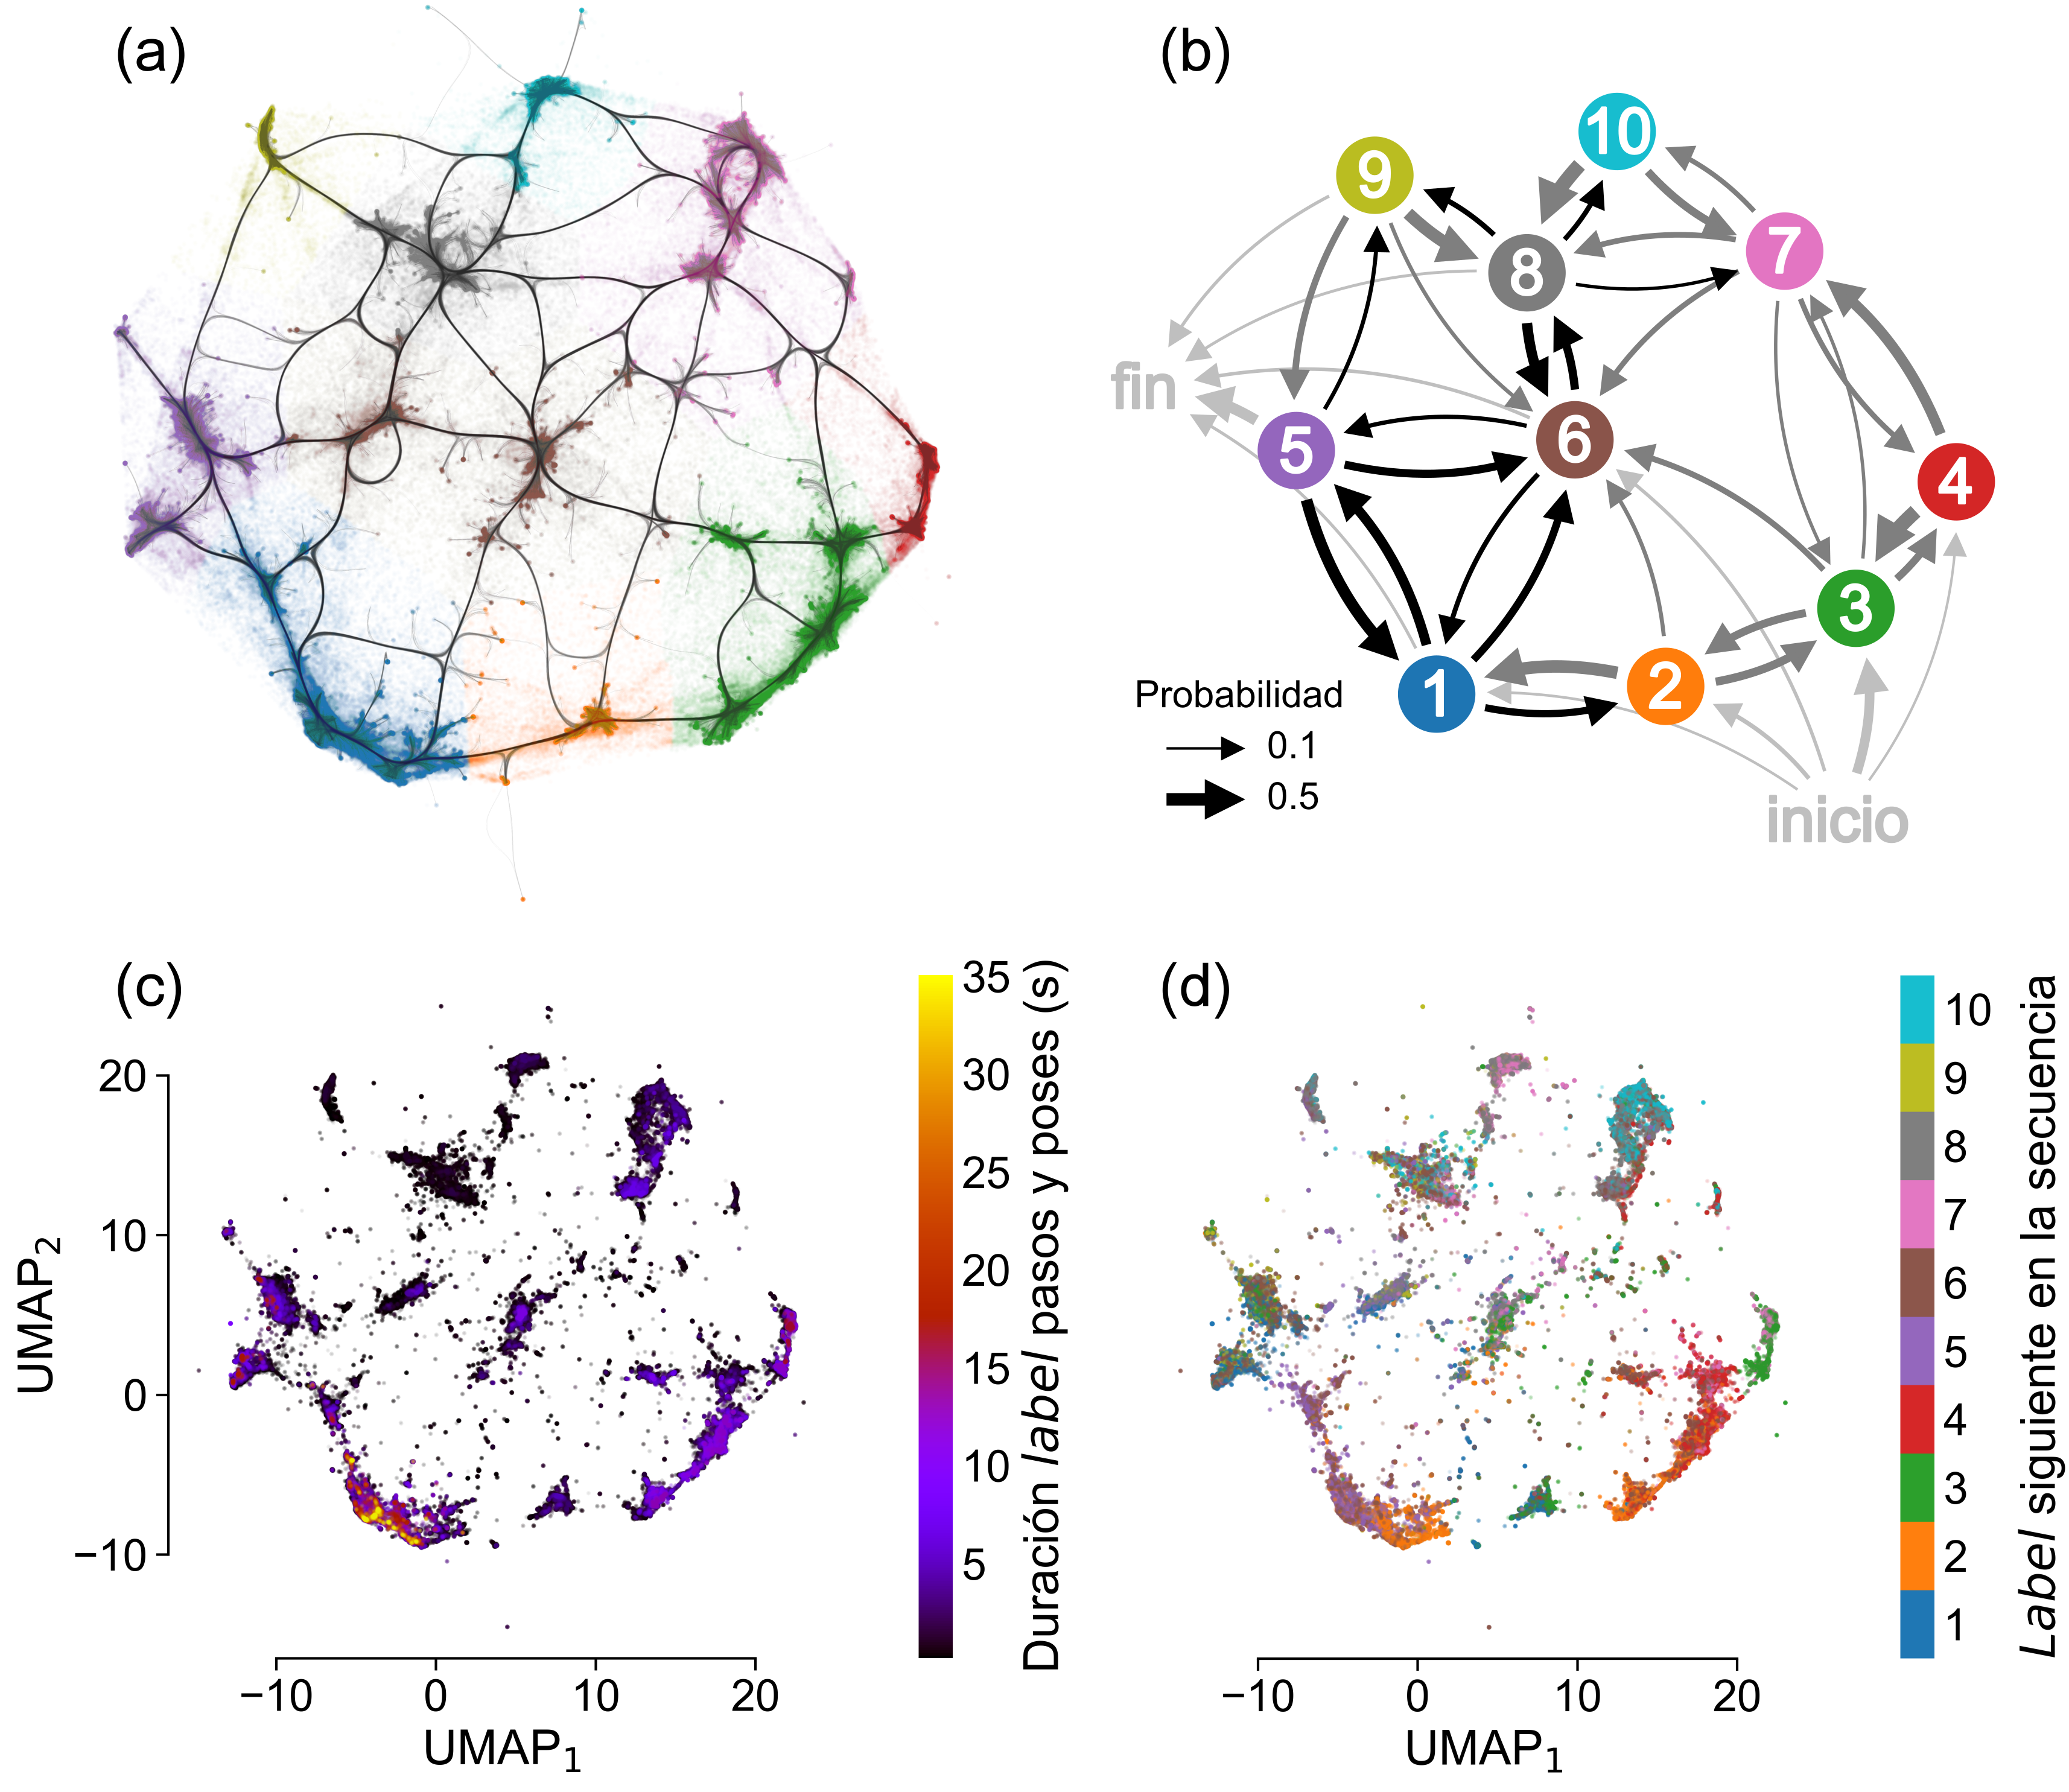
\includegraphics[width=0.99\linewidth]{figuras/capitulo4/labels_umap_stp.png}
    \caption{\textbf{\textit{Labels} de comportamiento de la proyección UMAP de las características de pasos y poses.}
        (a) Similaridad entre los puntos del mapa. El grosor de cada línea es proporcional a la similaridad entre las características de las regiones conectadas. (b) Grafo de transiciones temporales de las secuencias de \textit{labels}. El grosor de las flechas es proporcional a la probabilidad de transición. Sólo se muestran transiciones con probabilidad mayor al 10\%. Las flechas oscuras (grises) son transiciones desde un \textit{label} con probabilidad marginal en la secuencia mayor al 10\%. Las probabilidades de transición desde el estado ``inicio'' y hacia el estado ``fin'' fueron calculados \textit{ad hoc}. (c) Duración de cada \textit{label} en la secuencia según su ubicación en el mapa. (d) Descripción más fina de las transiciones en la secuencia de \textit{labels} según de qué ubicación en el mapa provengan.}
    \label{fig:capitulo4_labels_umap_stp}
\end{figure}

\clearpage

\section{Cambios en las secuencias de comportamiento}\label{sec:probabilidad_labels}

En principio, cada uno de los 10 ratones estudiados puede acceder, en un determinado instante de una prueba rotarod, a cualquiera de los estados comportamentales presentes en los mapas. Sin embargo, en la práctica los comportamientos representados en el mapa no son exhibidos por todos los individuos de la misma manera, y a su vez los repertorios comportamentales de cada individuo varían a lo largo del entrenamiento (Figuras \ref{fig:capitulo4_probabilidades_labels_wav} y \ref{fig:capitulo4_probabilidades_labels_stp}). En general, se observa que los \textit{labels} de pasos y poses separan más marcadamente a los ratones entre los grupos de alto y bajo rendimiento, comparados con los \textit{labels} \textit{wavelet}. Esto se debe a que las diferencias entre grupos de rendimiento aparecen como una estructura fina en la segmentación \textit{watershed} del mapa UMAP \textit{wavelet} (\autoref{fig:capitulo4_umap_wav}g). En otras palabras, los grupos de rendimiento están más mezclados de manera global en el mapa UMAP \textit{wavelet}, aunque pueden recuperarse las diferencias entre grupos si se accede a un nivel de detalle más fino. Mientras que en el mapa UMAP de pasos y poses hay una separación clara entre los grupos de rendimiento que fue mayormente capturada por la segmentación \textit{watershed} \textit{wavelet} (\autoref{fig:capitulo4_umap_stp}g). A grandes rasgos, esto indica que la dinámica global del movimiento de las partes del cuerpo de los ratones (espectros \textit{wavelet}) no es muy diferente entre grupos de rendimiento; mientras que en términos globales, las posiciones de las partes del cuerpo de los ratones en el cilindro y las características de sus pasos presentan diferencias más marcadas en comparación.

Para estudiar comportamientos bajo condiciones experimentales similares entre pruebas, analizamos la probabilidad de ocurrencia de \textit{labels} en los primeros 100 s de secuencias de comportamiento de cada prueba rotarod realizada. De esta manera, en el mapa UMAP \textit{wavelet}, los \textit{labels} 2 y 5 son exhibidos más frecuentemente por los ratones de bajo rendimiento y los \textit{labels} 9 y 10 por los de alto rendimiento. El resto, los \textit{labels} 1, 3, 4, 5, 6, 7, y 8 no son utilizados exclusivamente por ningún grupo de rendimiento (\autoref{fig:capitulo4_probabilidades_labels_wav}). Por su parte, en el mapa UMAP de pasos y poses, la diferencia entre grupos de rendimiento se manifiesta más fuertemente en la probabilidad de los \textit{labels} de comportamiento durante los primeros 100 s de las pruebas rotarod. Los \textit{labels} 1, 2, 5 y 6 son exhibidos preferentemente por los ratones de bajo rendimiento, mientras que los \textit{labels} 3, 4 y 7 son utilizados principalmente por los ratones de alto rendimiento. Solamente los \textit{labels} 8, 9 y 10 son utilizados en proporciones similares por ambos grupos de rendimiento (\autoref{fig:capitulo4_probabilidades_labels_stp}). De acuerdo a la interpretación del mapa de pasos y poses de la \autoref{fig:capitulo4_comentario_label_umap}b, los ratones de bajo rendimiento tienden a dar pasos de mayor velocidad, presentan menor desfasaje entre sus patas traseras (o sea que las levantan más o menos al mismo tiempo), se mueven a alturas más bajas sobre el cilindro y dan pasos a menor frecuencia (o sea que dejan pasar más tiempo entre pasos consecutivos y son arrastrados una distancia mayor por la rotación del cilindro). En comparación, los ratones de alto rendimiento dan pasos más cortos a menor velocidad, manteniéndose en la parte superior del cilindro la mayor parte del tiempo, con tendencia a un mayor desfasaje entre sus pasos (es decir, tienen una locomoción más alternante). Muchas de las probabilidades de \textit{label} en la secuencia varían significativamente a lo largo de los días de entrenamiento, a juzgar por los p-valores de test \textit{one-way} ANOVA (Figuras \ref{fig:capitulo4_probabilidades_labels_wav} y \ref{fig:capitulo4_probabilidades_labels_stp}). En muchos casos se observa además una gran variabilidad intra-día en las probabilidades de \textit{label} en los primeros 100 s de las secuencias de comportamiento. En consecuencia, la gran variabilidad intra-día reduce la significancia estadística de la variación de estas métricas durante el entrenamiento, especialmente para el grupo de 3 ratones de alto rendimiento comparado con el grupo de 7 ratones de bajo rendimiento. A pesar de esto, se observa en términos generales una reducción en la variabilidad intra-día de las probabilidades de los \textit{labels}, indicando que con el entrenamiento se afianza la ejecución de ciertos tipos de comportamiento con mayor precisión.

En resumen, se observa una estructura temporal en las secuencias de labels, existiendo una marcada preferencia por iniciar y terminar las pruebas rotarod usando categorías de comportamientos diferentes. Los \textit{labels} de pasos y poses separan más fuertemente a los ratones según su grupo de rendimiento, comparados con los \textit{labels} \textit{wavelet}. Esto puede deberse a que los espectros wavelets presentan más invarianzas, matemáticamente hablando, que las características de pasos y poses. Específicamente, los espectros wavelet de los ángulos de las partes del cuerpo de los ratones son invariantes ante pequeñas rotaciones rígidas, traslaciones espacio-temporales y cambios de escala en el cuerpo de los ratones, por lo que tiene sentido que separen menos a los ratones individualmente al ser características que generalizan mejor.

Se observa que la variabilidad en las probabilidades de labels durante los primeros 100 s de las secuencias de comportamiento se reduce con el entrenamiento. Esto se observa a través de la entropía de las secuencias (\autoref{fig:capitulo4_entropia}), la cual se reduce significativamente para ambos grupos de rendimiento en el caso de los \textit{labels wavelet} (\autoref{fig:capitulo4_entropia}a) y significativamente para los 7 ratones de bajo rendimiento en los \textit{labels} de pasos y poses (\autoref{fig:capitulo4_entropia}b). Para ambos tipos de \textit{labels} no se observan diferencias significativas entre los grupos de rendimiento en los valores de las entropías. Sin embargo, la entropía de los comportamientos de los 3 ratones de alto rendimiento es ligeramente inferior durante todo el entrenamiento. La entropía de las proyecciones UMAP también se reduce con los días de entrenamiento (Figuras \ref{fig:capitulo4_umap_wav}h y \ref{fig:capitulo4_umap_stp}h suplementarias). Sosteniendo que la variabilidad en las estrategias de comportamiento usadas por los ratones se reduce con el aprendizaje. El uso de mapas UMAP de dimensión reducida permite un enfoque holístico en el estudio del comportamiento: permite estudiar los efectos y cambios de múltiples características comportamentales simultáneamente en una conveniente representación de fácil visualización.

\begin{figure}[htbp]
    \centering
    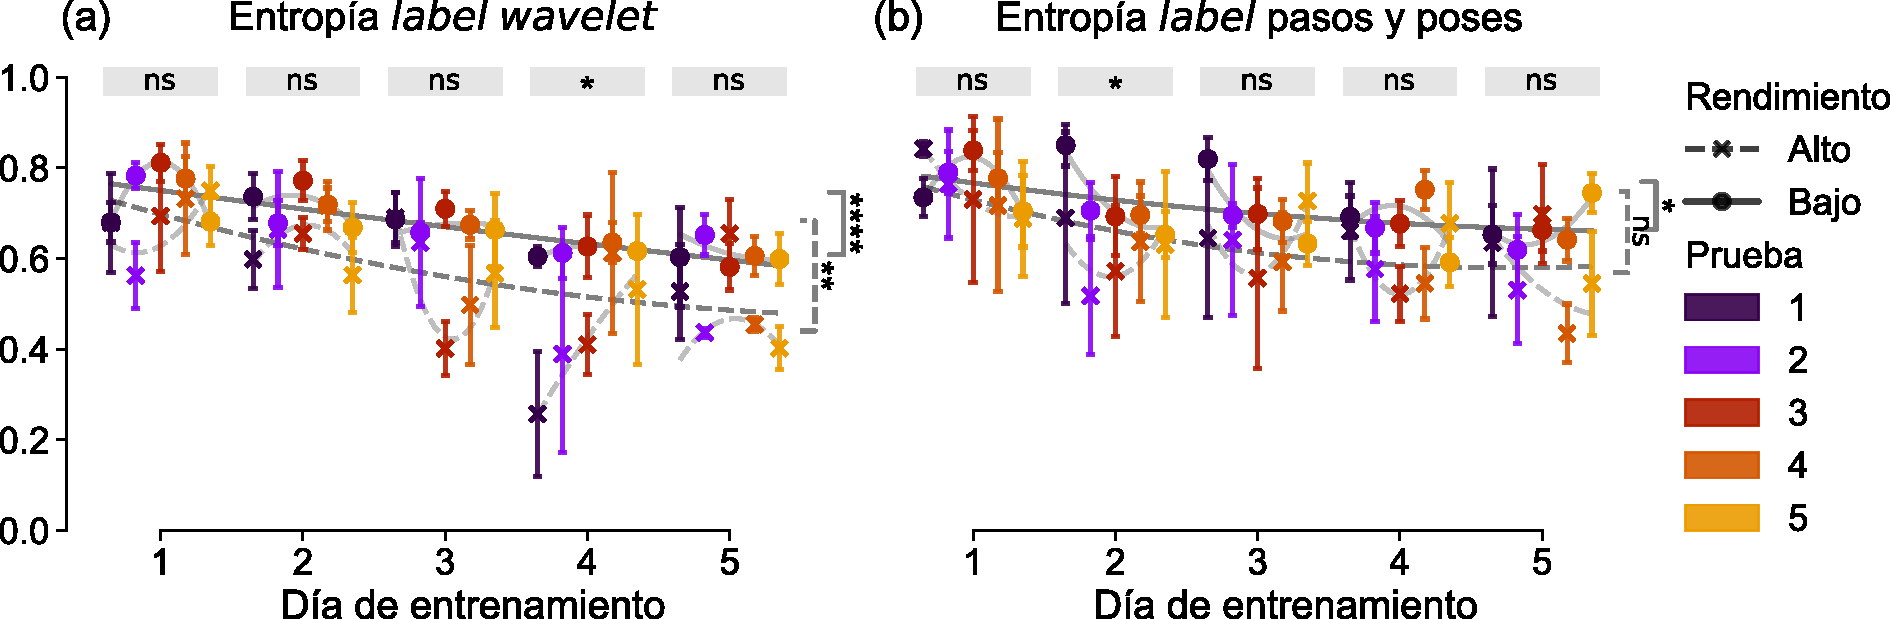
\includegraphics[width=0.99\linewidth]{figuras/capitulo4/entropia.pdf}
    \caption{\textbf{Entropía de las secuencias de \textit{labels}.}
        Entropía de las secuencias de comportamientos durante los primeros 100 s de las pruebas rotarod, para cada día de entrenamiento y número de prueba realizada ese día. Las entropías son relativas a la entropía máxima dada por la distribución marginal de los \textit{labels} en las secuencias. Los puntos muestran el promedio por grupo de rendimiento y las barras son el error estándar del promedio. Los rectángulos grises, en el margen superior de cada subfigura, indican los p-valores T-test entre grupos de rendimiento para cada día. Los corchetes en los márgenes derechos indican, para cada grupo de rendimiento, los p-valores \textit{one-way} ANOVA agrupando por día de entrenamiento. (a) \textit{Labels wavelet}. (b) \textit{Labels} pasos y poses.}
    \label{fig:capitulo4_entropia}
\end{figure}

\begin{figure}[htbp]
    \centering
    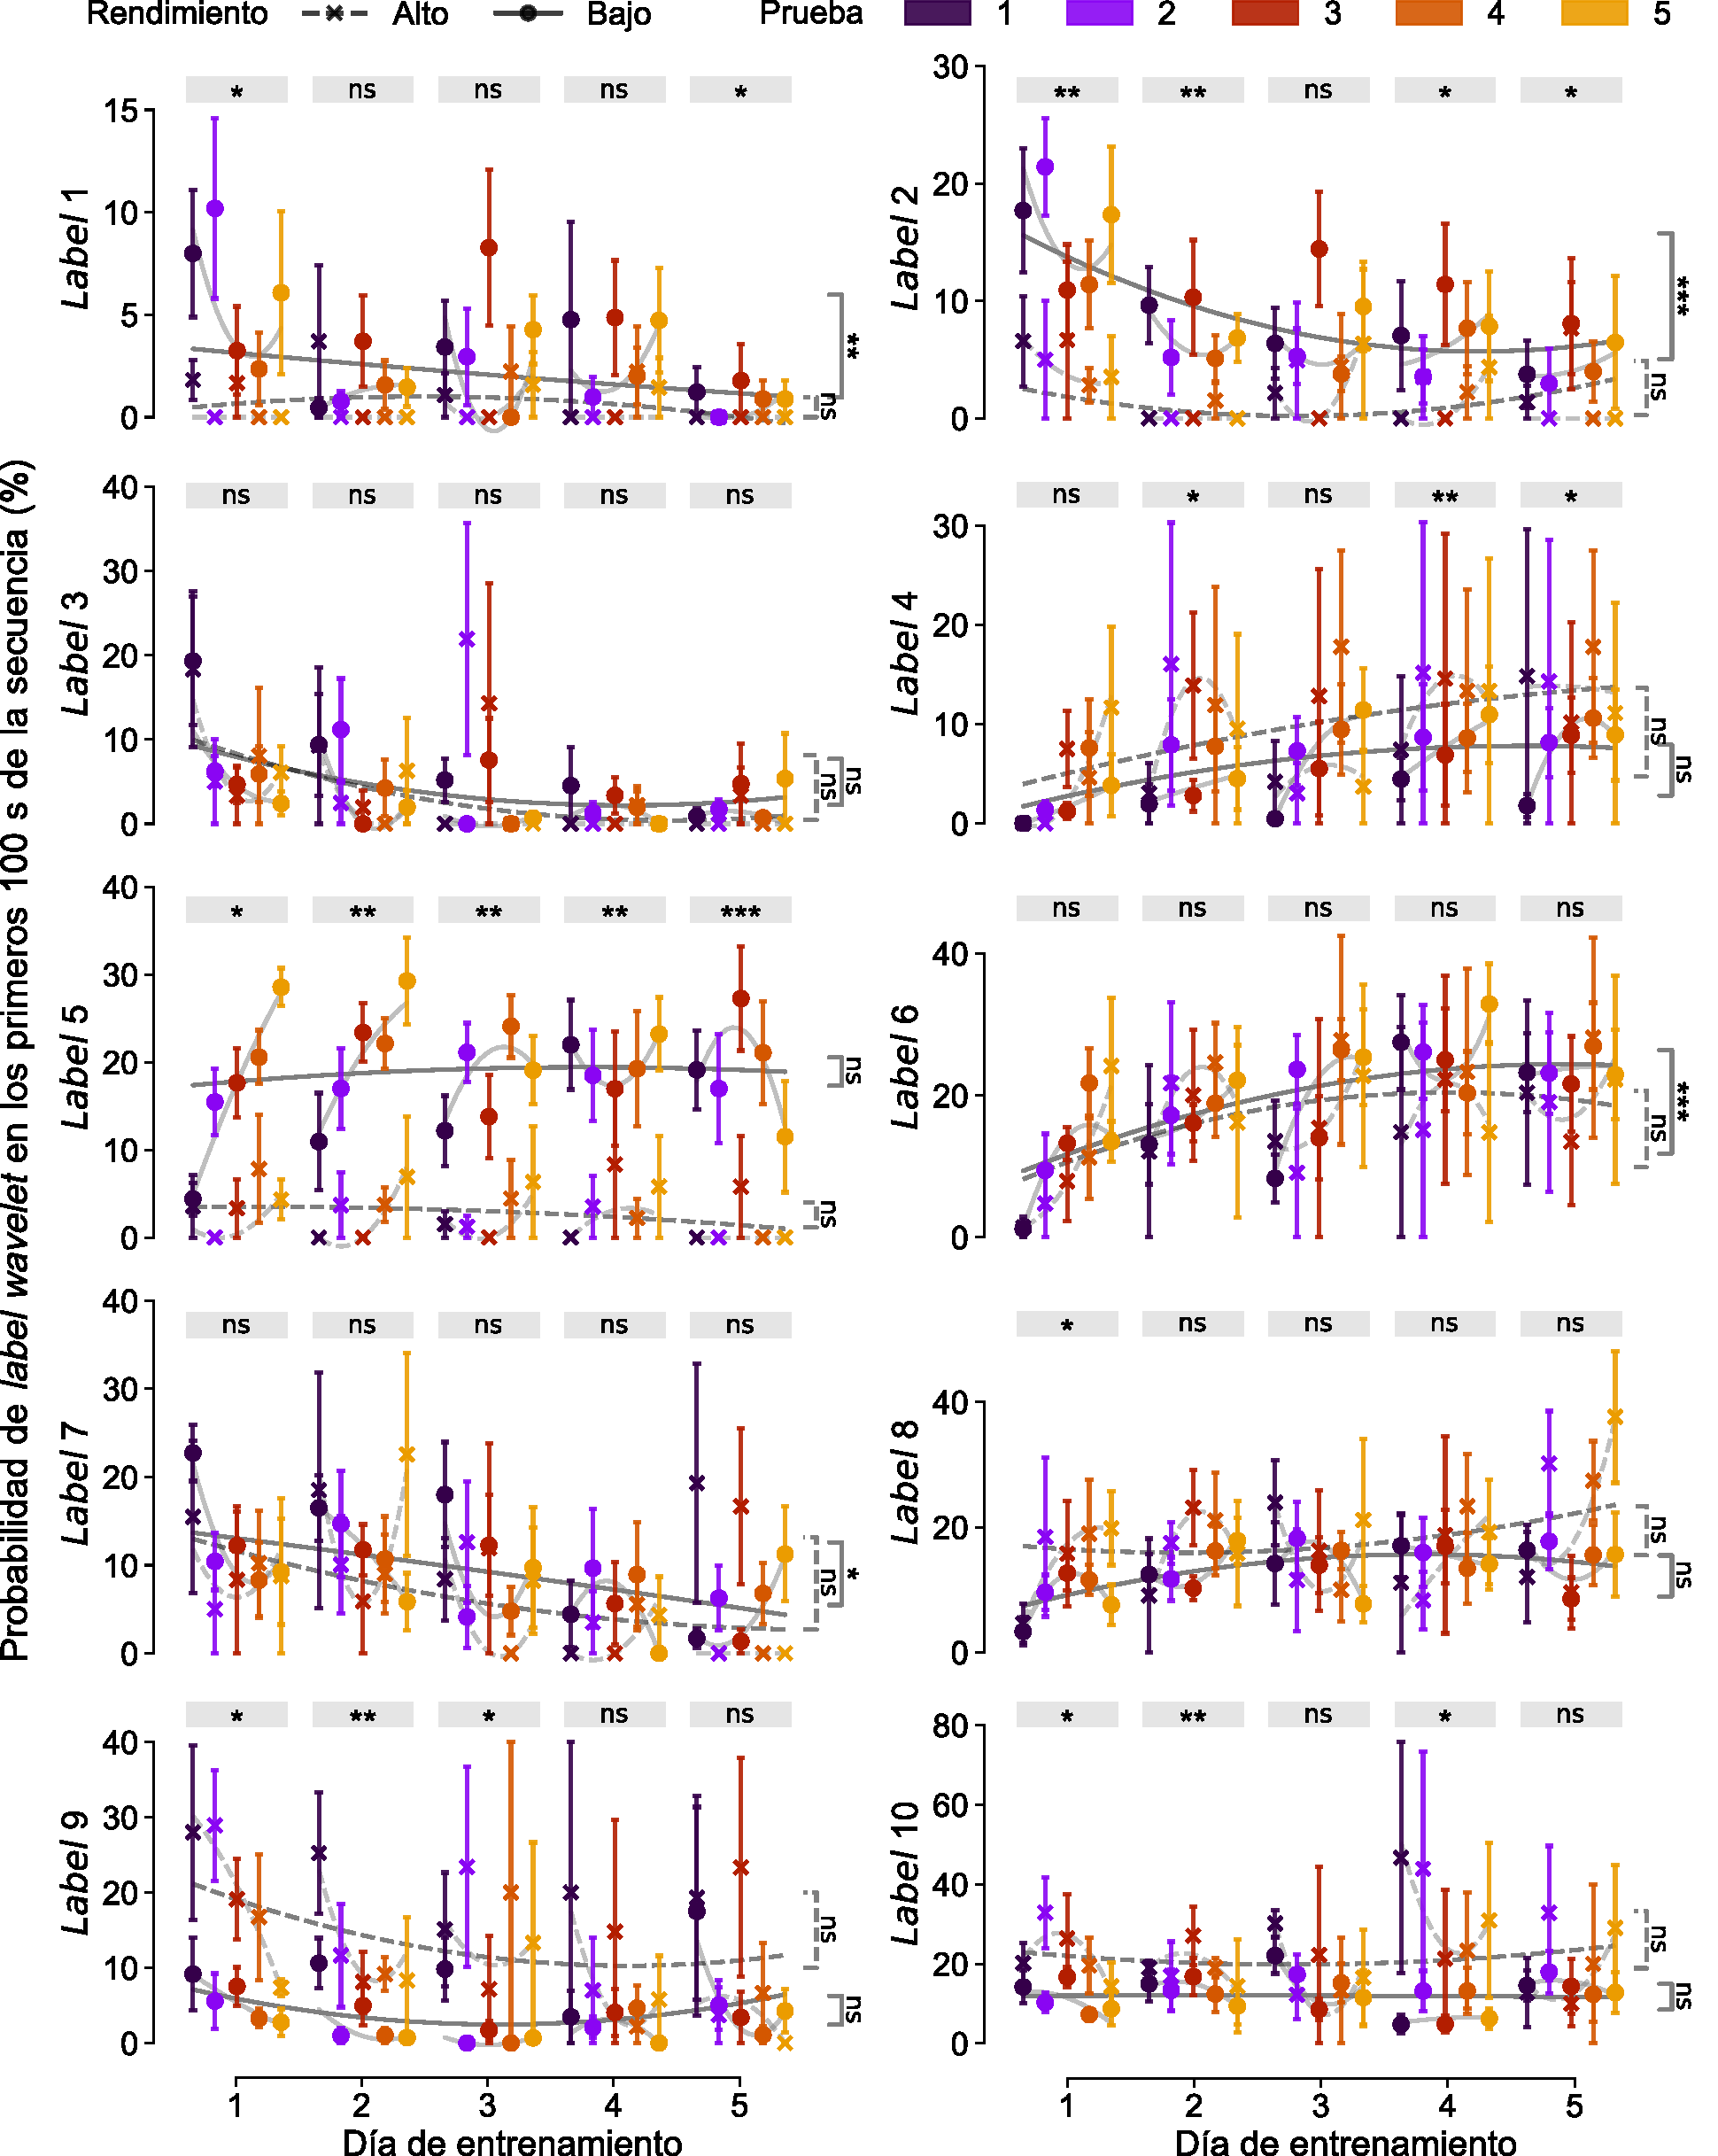
\includegraphics[width=0.99\linewidth]{figuras/capitulo4/probabilidades_labels_wav.pdf}
    \caption{\textbf{Cambios en las probabilidades de \textit{label} \textit{wavelet} en las secuencias de comportamiento.} Cada subfigura de la grilla representa la probabilidad de ocurrencia de un determinado \textit{label} durante los primeros 100 s de las pruebas rotarod, para cada día de entrenamiento y número de prueba realizada ese día. Los puntos muestran el promedio por grupo de rendimiento y las barras son el error estándar del promedio. Los rectángulos grises, en el margen superior de cada subfigura, indican los p-valores T-test entre grupos de rendimiento para cada día. Los corchetes en los márgenes derechos indican, para cada grupo de rendimiento, los p-valores \textit{one-way} ANOVA agrupando por día de entrenamiento.}
    \label{fig:capitulo4_probabilidades_labels_wav}
\end{figure}

\begin{figure}[htbp]
    \centering
    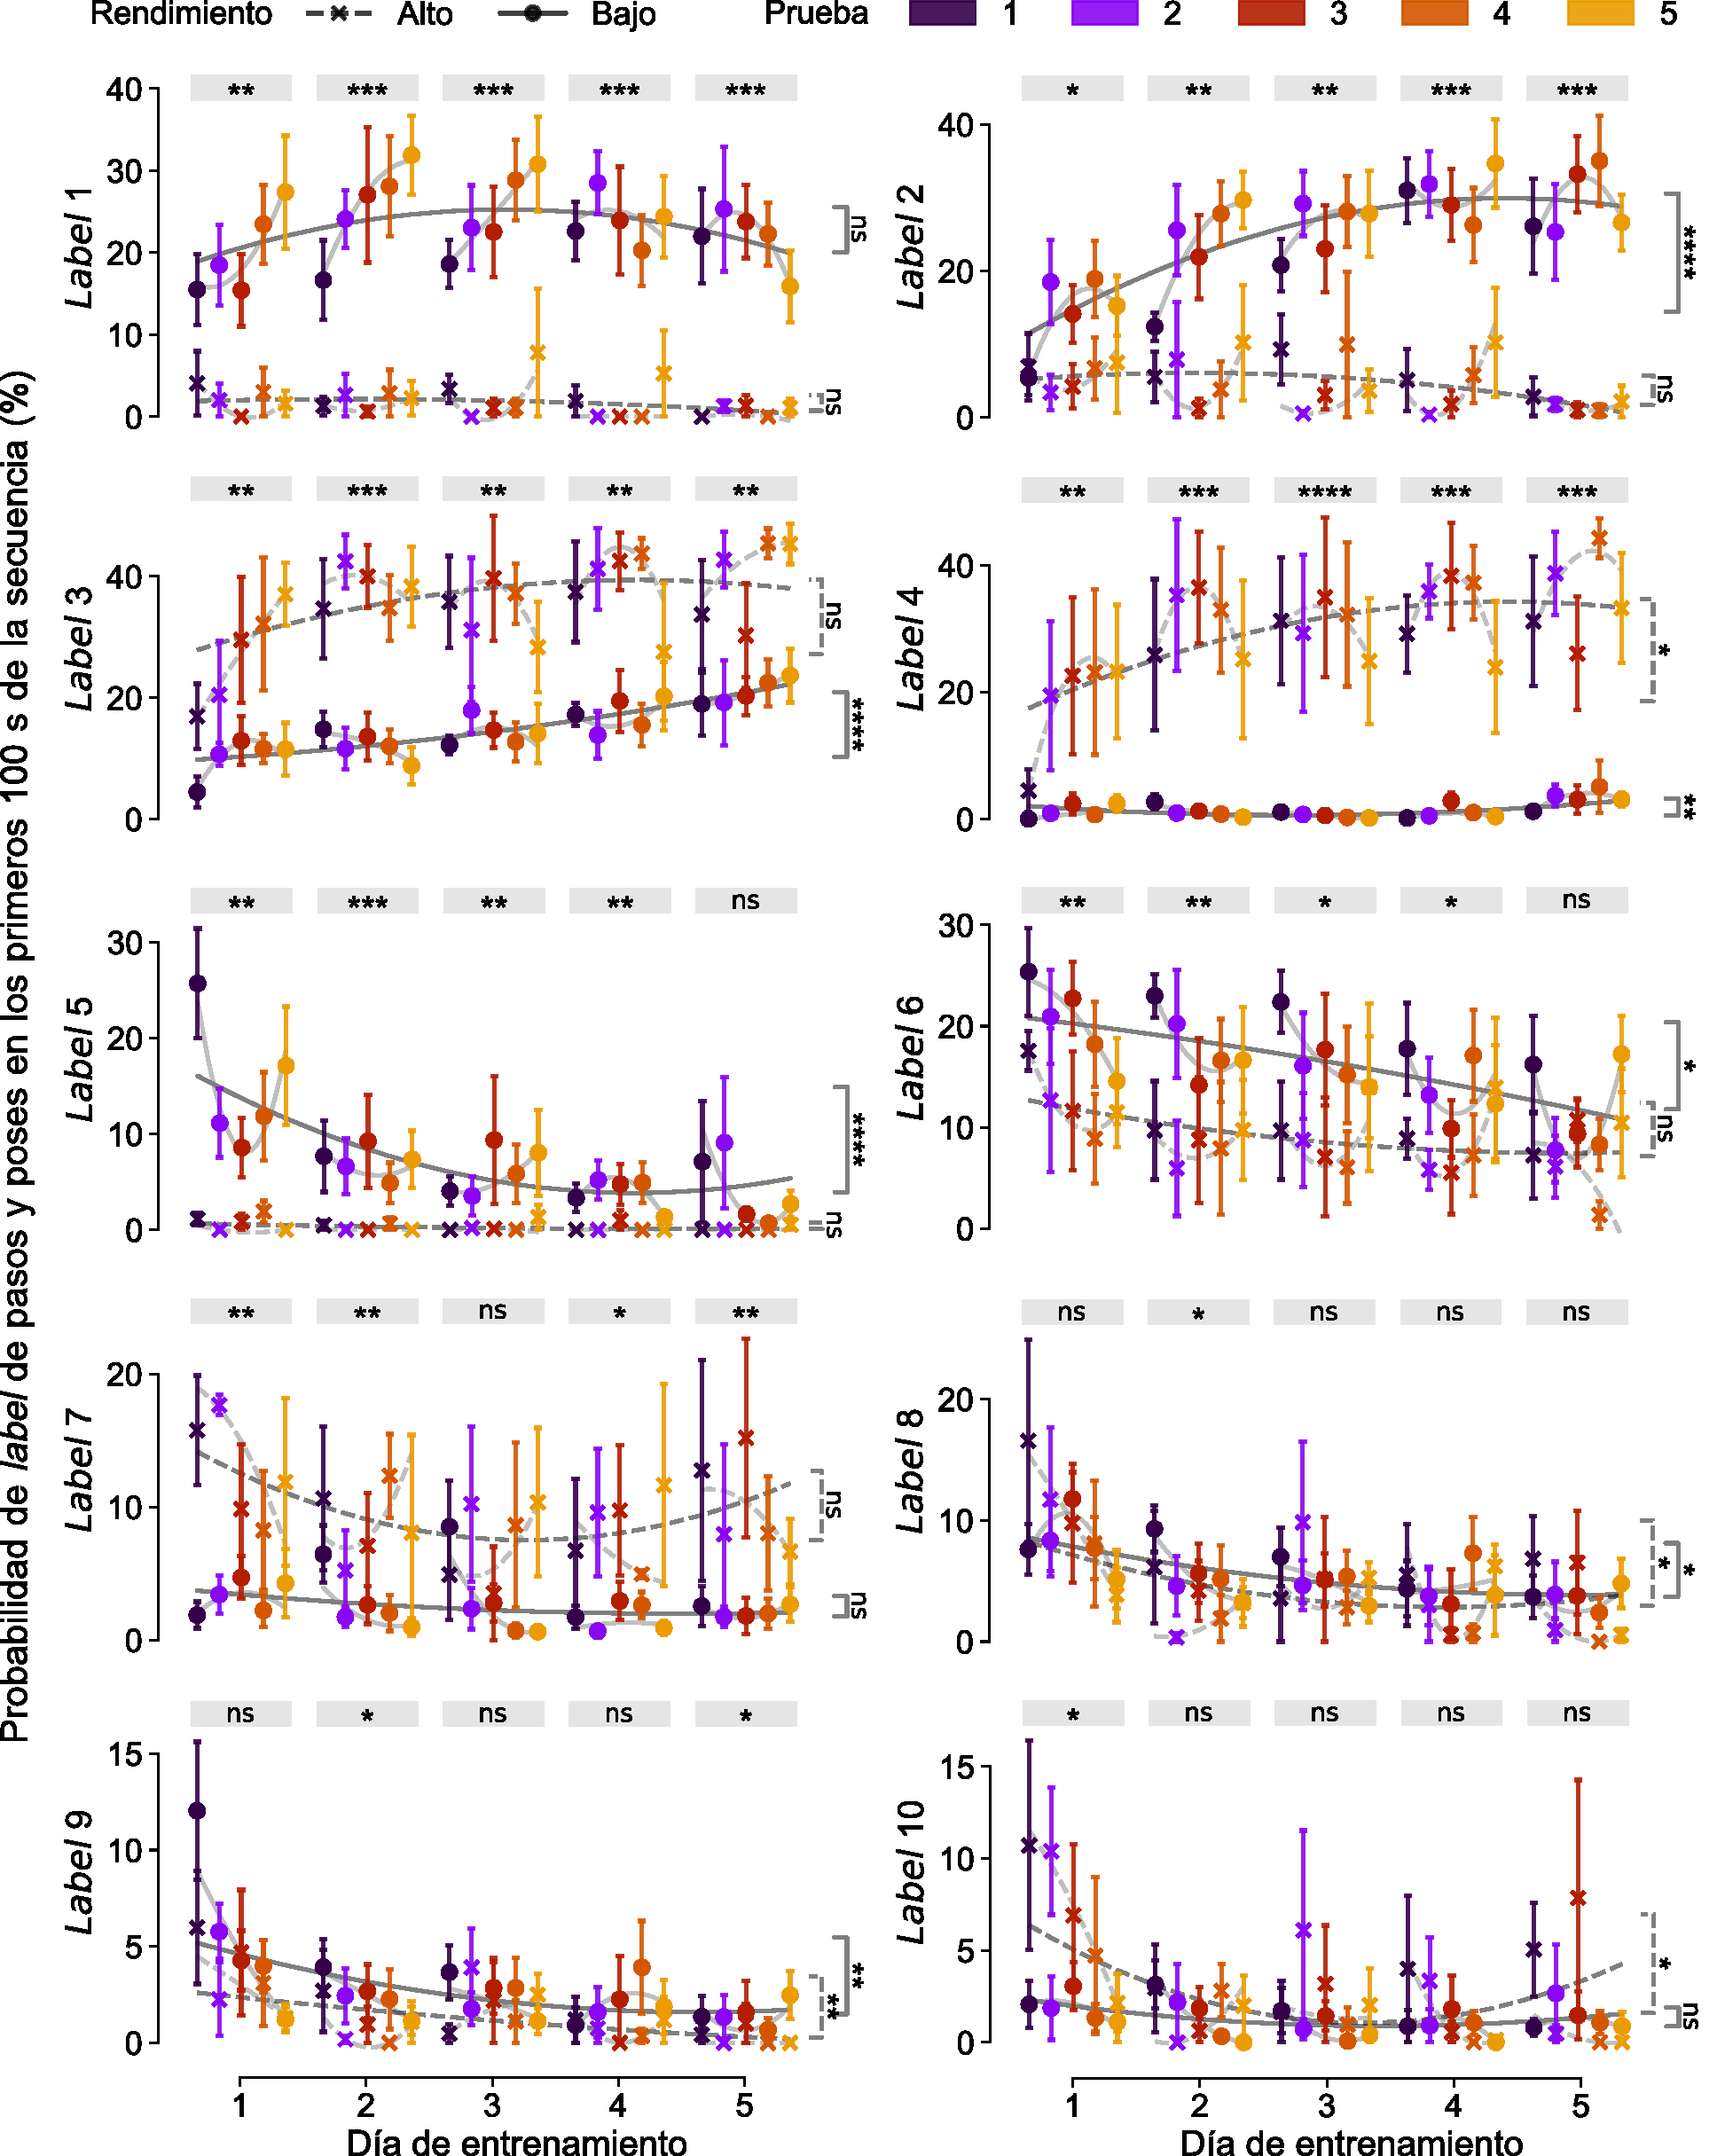
\includegraphics[width=0.99\linewidth]{figuras/capitulo4/probabilidades_labels_stp.pdf}
    \caption{\textbf{Cambios en las probabilidades de \textit{label} de pasos y poses en las secuencias de comportamiento.} Cada subfigura de la grilla representa la probabilidad de ocurrencia de un determinado \textit{label} durante los primeros 100 s de las pruebas rotarod, para cada día de entrenamiento y número de prueba realizada ese día. Los puntos muestran el promedio por grupo de rendimiento y las barras son el error estándar del promedio. Los rectángulos grises, en el margen superior de cada subfigura, indican los p-valores T-test entre grupos de rendimiento para cada día. Los corchetes en los márgenes derechos indican, para cada grupo de rendimiento, los p-valores \textit{one-way} ANOVA agrupando por día de entrenamiento.}
    \label{fig:capitulo4_probabilidades_labels_stp}
\end{figure}